\documentclass[a4paper, 12pt]{report}
\usepackage{graphicx}
\usepackage[utf8]{inputenc}
\usepackage{graphicx}
\usepackage{fancyhdr}
\usepackage[english]{babel}

\newcommand{\myparagraph}[1]{\paragraph{#1}\mbox{}\newline\\}

\title{Rapport de Stage}
\author{Pierre De Abreu}
\date{February, 8th 2016 - August, 8th 2016}

\newcommand{\HRule}{\rule{\linewidth}{0.5mm}}
 
\pagestyle{fancy}
\fancyhf{}
\rhead{Sogeti, ESEC}
\lhead{EPITA / SRS 2016}
\rfoot{
\includegraphics[width=4cm]{images/esec-footer.png}}
\lfoot{
\includegraphics[width=2cm]{images/epita.png}}
\lfoot{
\includegraphics[width=2cm]{images/srs.png}}
\cfoot{\thepage}
 
\begin{document}
\begin{titlepage}
\begin{center}

% Upper part of the page. The '~' is needed because \\
% only works if a paragraph has started.

\includegraphics[width=0.3\textwidth]{images/epita.png}~\\[1cm]

\textsc{\LARGE EPITA / SRS 2016}\\[1.5cm]

\textsc{\Large  Internship}\\[0.5cm]
\textsc{\Large 08/02/2016 - 08/08/2016}

% Title
\HRule \\[0.4cm]
{ \huge \bfseries Sogeti, ESEC \\[0.4cm] }

\HRule \\[1.5cm]

% Author and supervisor
\begin{minipage}{0.4\textwidth}
\begin{flushleft} \large
\emph{Author:}\\
Pierre \textsc{De Abreu (UID: 66101)}
\end{flushleft}
\end{minipage}
\begin{minipage}{0.4\textwidth}
\begin{flushright} \large
\emph{Supervisor:} \\
Adrien \textsc{Fay}
\end{flushright}
\end{minipage}


\includegraphics[width=0.5\textwidth]{images/esec.png}~\\[1cm]

\vfill

% Bottom of the page
\end{center}
\end{titlepage}
\section*{Sogeti and ESEC}
Sogeti is a digital services company, belonging to the Capgemini group. It has been created in 1967 in Grenoble (France) by Serge Kampf, and now has missions in 15 countries with more than 25 000 employees, around 6200 of them working in France.
\section*{Service}
ESEC (which stands for European Security Expertise Center) is the TODO of Sogeti. It is divided in several teams (R\&D laboratory, penetration testing team, etc.). This internship took place in the penetration testing team.
The current director of all the security services of Capgemini is Frank Greverie, and the Jean Marc Bianchini is directing the ESEC for Sogeti.
Adrien Fay, the supervisor of this internship, is working in the penetration testing team, which is leaded by Guillaume Meunier. After its studies in Grenoble, Adrien started an internship in Sogeti, and stayed there at the end.
\section*{My work}
This internship final goal was to develop a static analyzer in Python to detect use-after-free vulnerabilities. It started by studying how memory allocator are designed on both Linux and Windows (especially the look-aside lists and latter the Low Fragmentation Heap mechanismes on Windows). The second part was to understand how these design flaws could lead to use-after-free vulnerabilities exploitation. Then, two weeks were dedicated to practical cases with known vulnerabilities on old and new versions of Windows.\subparagraph{}
The last part was the actual development of the tool. A base security framework had to be chosen, and then the design of the tool had to be decided. Finally, the developpement started with a skeleton to walk through the binary given as input, then an use-after-free basic detection was implemented. The optimisation of the binary traversal was the last thing and took the last month of this internship.
\section*{Existing state of affair}
Several tools already exist, whether they are dynamic or static analysers.
\myparagraph{Dynamic analysers}
Kasan (Kernel Address Sanitizer) and Adress Sanitizer are two good examples of what already exist on the dynamic side. They both need to compile source code with some specific options and libraries and then output errors if use-after-free bugs happen when the program is running.
\myparagraph{Static analysers}
GUEB has been developped by Josselin Feist during his thesis. This tools uses information given by BinNavi to walk through the binary and find vulnerabilities.
\myparagraph{Static versus Dynamic}
Both have pro and cons. Dynamic analysis is somehow easier since the progam is actually running, thus making the allocated addresses and size available to the analyser. Path exploration is easier since it is determined by the set of input given to the analyser. But dynamic analyser lack the ability to be complete in a path covering manners. It can only explore paths the input given to it allow.
\subparagraph{}
Static analysys can explore all the possible path, but do not know the actual size or addresses returned by allocation. It makes branching harder since dynamic value may be restricted in a way the analyser doesn't know, thus leading to the exploration of a path that could not be taken in real life. It also leads to path explosion problem, because every branching and loop must be simulated, and deciding when to leave a loop is not trivial. It also takes a lot of time and uses a lot of memory space due to this simulation.

\newpage
\section*{Timeline}
\begin{figure}[h]
\begin{center}
    \rotatebox{90}{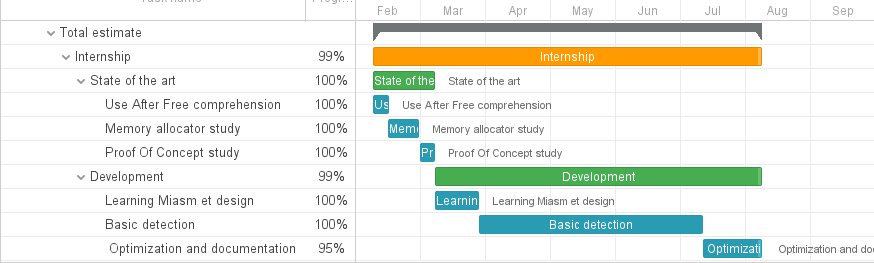
\includegraphics[scale=0.46]{images/gantt-english.png}}\newline
    \caption{Timeline}
\end{center}
\end{figure}
Everything went as planned. During the "PoC study" part, it was not important if the ongoing work was stopped, since it was only a bonus in the discovery of use-after-free vulnerabilities.
\section*{General appreciation and working conditions}
This internship gave me the opportunity to work on subjects I had never experienced before, like symbolic execution, SMT solver or static analysis. The graph theory part of the development was also more difficult than what I used to work on at school.
I was free to implement the tool as I wanted to, the only constraint was for it to be modular and documented, in a way it would be easier for an other person to come after me and work on it.
The team was really nice, and it did not take a long time before I felt comfortable. Every intern had a laptop, a second screen and his own desk from the very first day, and people were always open to questions.
\section*{Skills}
This internship asked from me the following skills:
\begin{itemize}
        \item Python
        \item Security static analysis
        \item Graph theory
        \item Symbolic execution
        \item SMT solver and constraints solving
        \item Optimization and software design
\end{itemize}
\section*{Conclusion}
This 6 months in Sogeti were really a good experience, as I learned new things and improved my already existing skills. The environment was just fine, and I did feel comfortable in the penetration testing team. Being with them at all time also teached me how it was to work for a digital services company.
I would like to thank my supervisor Adrien Fay, as well as the penetration testing team manager, Guillaume Meunier, for their presence and their answer to all my questions.

\end{document}
